\documentclass{article}
\usepackage[T1]{fontenc}
\usepackage{lmodern}
\usepackage{graphicx}
\usepackage{amsmath,amssymb}
\usepackage[a4paper,margin=2cm]{geometry}
\usepackage[absolute,overlay]{textpos}
\setlength{\TPHorizModule}{1mm}
\setlength{\TPVertModule}{1mm}
\usepackage[indonesian]{babel}
\usepackage{hyperref}
\setlength{\emergencystretch}{2em}
% unit: Halaman 63

\begin{document}

% === Halaman 63 (llm) ===

\vspace{219.78mm}

Contoh sebuah full Vigen\`ere square

% deskripsi: Tabel Vigen\`ere square yang berisi alfabet A-Z pada baris dan kolom, dengan setiap sel berisi karakter hasil enkripsi pergeseran alfabet.
% bbox normalisasi: [0.2900, 0.2300, 0.7400, 0.9700]
\begin{textblock*}{94.50mm}(60.90mm,68.31mm)
\noindent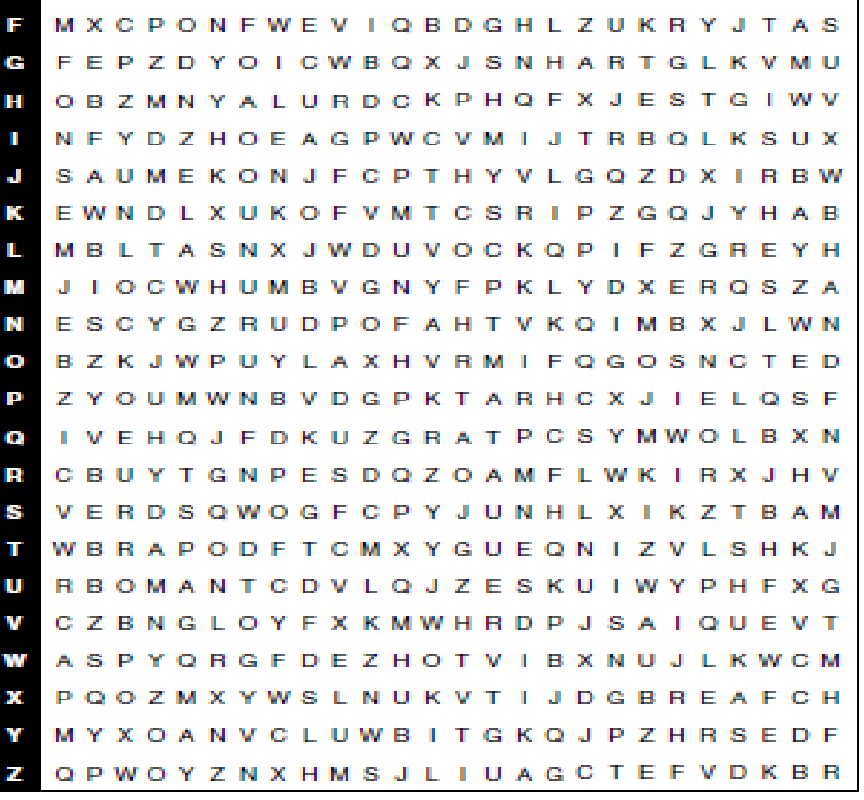
\includegraphics[width=94.50mm,height=219.78mm]{../../images/llm/page_063_img_01.png}%
\end{textblock*}

\end{document}
